\documentclass[17pt]{beamer}
\usepackage{amsmath}
\usepackage{framed}
\definecolor{Blue}{RGB}{0.16,0.32,0.75}
\setbeamercolor{structure}{fg=blue}
\usepackage{beamerthemesplit}




\definecolor{blue}{rgb}{0.16,0.32,0.75}
\setbeamercolor{structure}{fg=blue}
\author[FOSSEE]{}
\institute[IIT Bombay]{}
\date[]{}
% \setbeamercovered{transparent}

% theme split
\usepackage{verbatim}
\newenvironment{colorverbatim}[1][]%
{%
	\color{blue}
	\verbatim
}%
{%
	\endverbatim
}%

\usepackage{mathpazo,courier,euler}
\usepackage{listings}
\lstset{language=sh,
	basicstyle=\ttfamily\bfseries,
	showstringspaces=false,
	keywordstyle=\color{black}\bfseries}

% logo
\logo{
\includegraphics[height=1.30 cm]{St-logo.png}}
\logo{
\includegraphics[height=1.30 cm]{fossee-logo.png}
	
	\hspace{7.5cm}
	
\includegraphics[scale=0.3]{fossee-logo.png}\\
	\hspace{281pt}
	
\includegraphics[scale=0.08]{St-logo.png}}


\newcounter{saveenumi}
\newcommand{\seti}{\setcounter{saveenumi}{\value{enumi}}}
\newcommand{\conti}{\setcounter{enumi}{\value{saveenumi}}}

\begin{document}
	% sf family, bold font
	\sffamily \bfseries
	%\LARGE
	\title
	[Python for Scientific Computing]
	%\hspace{0.5cm}
	%\insertframenumber/\inserttotalframenumber]
	{\large Using Python Modules}
	\author
	[FOSSEE, IIT Bombay]
	{{\small Spoken Tutorial Project \\ http://spoken-tutorial.org \\ National Mission on Education  through ICT  \\ http://sakshat.ac.in } \\
		{\small Script: Thirumalesh H S}\\
		{\small Narrator: Kiran Kishore}\\
		{\small IIT Bombay}\\
		{\small 21 December 2015}}
	
	% slide 1
	\begin{frame}
		\titlepage
	\end{frame}
%%%%%%%%%%%%%%%%%%%%%%%%%%%%%%%%%%%%%%%%%%%%%%%%%%%%%%%%%%%%%%%%%%%%%%%%%%%%%%%%
\begin{frame}
\frametitle{Objectives}
\label{sec-2}

  At the end of this tutorial, you will be able to- \pause

\begin{itemize}
\item Execute python scripts from command line.\pause
\item Use import in scripts.\pause
\item Import scipy and pylab modules.\pause
\item Use python standard modules and 3rd party modules.
\end{itemize}
\end{frame}
%%%%%%%%%%%%%%%%%%%%%%%%%%%%%%%%%%%%%%%%%%%%%%%%%%%%%%%%%%%%%%%%%%%%%%%%%%%%%%%%
\begin{frame}
\frametitle{System Specifications}\pause
\begin{itemize}
\item Ubuntu Linux 14.04\pause
\item \texttt{Python 2.7.6} \pause
\item \texttt{IPython 4.0.0}
\end{itemize}
\end{frame}
%%%%%%%%%%%%%%%%%%%%%%%%%%%%%%%%%%%%%%%%%%%%%%%%%%%%%%%%%%%%%%%%%%%%%%%%%%%%%%%%
\begin{frame}
	\frametitle{Pre-requisite}
	\label{sec-3}
	
	To practice this tutorial, you should know how to -\pause
	
	\begin{itemize}
		\item use plot interactively \pause
		\item embellish and save a plot \pause
	\end{itemize}
	If not, see the pre-requisite Python tutorials on {\color{blue}http://spoken-tutorial.org}
\end{frame}
%%%%%%%%%%%%%%%%%%%%%%%%%%%%%%%%%%%%%%%%%%%%%%%%%%%%%%%%%%%%%%%%%%%%%%%%%%%%%%%%
\begin{frame}[fragile]
\frametitle{Running Python script from command line}
\label{sec-4}

\begin{itemize}
\item Create a simple python script to print hello world. 
\end{itemize}
\end{frame}
%%%%%%%%%%%%%%%%%%%%%%%%%%%%%%%%%%%%%%%%%%%%%%%%%%%%%%%%%%%%%%%%%%%%%%%%%%%%%%%%
\begin{frame}
\frametitle{Four plot problem}
\label{sec-6}

    \begin{center}
      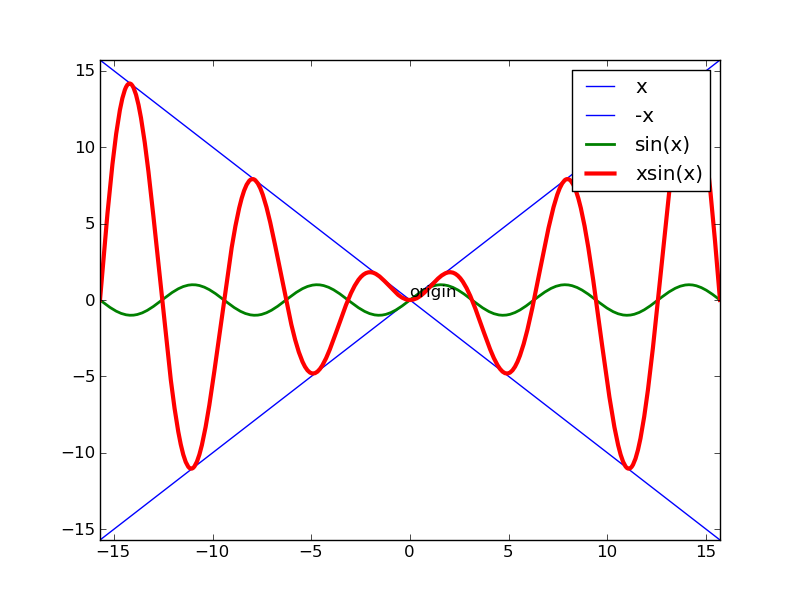
\includegraphics[scale=0.4]{four_plot}    
    \end{center}
\end{frame}
%%%%%%%%%%%%%%%%%%%%%%%%%%%%%%%%%%%%%%%%%%%%%%%%%%%%%%%%%%%%%%%%%%%%%%%%%%%%%%%%
\begin{frame}[fragile]
\frametitle{Fix \texttt{linspace()} problem}
\label{sec-7}

\texttt{from scipy import *}
\end{frame}
%%%%%%%%%%%%%%%%%%%%%%%%%%%%%%%%%%%%%%%%%%%%%%%%%%%%%%%%%%%%%%%%%%%%%%%%%%%%%%%%
\begin{frame}[fragile]
\frametitle{Better way of fixing}
\label{sec-9}

\texttt{from scipy import linspace}\\\pause
\vspace{5pt}
  instead of\\\pause
\vspace{5pt}
\texttt{from scipy import *}\\\pause
\vspace{5pt}
\texttt{*} means import all functions from name-space \texttt{scipy}.
\end{frame}
%%%%%%%%%%%%%%%%%%%%%%%%%%%%%%%%%%%%%%%%%%%%%%%%%%%%%%%%%%%%%%%%%%%%%%%%%%%%%%%%
\begin{frame}[fragile]
\frametitle{Another Fix}
\label{sec-11}

\begin{itemize}
	\item Open the script another-fix.py\pause
	\item Run the script another-fix.py
\end{itemize}
\end{frame}
%%%%%%%%%%%%%%%%%%%%%%%%%%%%%%%%%%%%%%%%%%%%%%%%%%%%%%%%%%%%%%%%%%%%%%%%%%%%%%%%
\begin{frame}
\frametitle{Assignment 1}
\label{sec-12}

\begin{itemize}
\item Write a python script to plot a sine wave from 
    $-2\pi$
  to 
    $2\pi$
  .
\end{itemize}
\end{frame}
%%%%%%%%%%%%%%%%%%%%%%%%%%%%%%%%%%%%%%%%%%%%%%%%%%%%%%%%%%%%%%%%%%%%%%%%%%%%%%%%
\begin{frame}
\frametitle{What is a module?}
\label{sec-13}
\begin{itemize}
\item Module is simply a file containing Python definitions and
  statements.\pause
\item Definitions from a module can be imported into other
  modules or into the main module.
\end{itemize}
  
\end{frame}
%%%%%%%%%%%%%%%%%%%%%%%%%%%%%%%%%%%%%%%%%%%%%%%%%%%%%%%%%%%%%%%%%%%%%%%%%%%%%%%%
\begin{frame}
\frametitle{Python standard library}
\label{sec-14.1}

  Python has a very rich standard library of modules.\pause

\begin{itemize}
\item Some of the standard modules are,
	\begin{itemize}
	\item Math: \texttt{math}, \texttt{random}\pause
	\item Internet access: \texttt{urllib2}, \texttt{smtplib}\pause
	\item System, Command line arguments: \texttt{sys}
	\end{itemize}
\end{itemize}
\end{frame}
%%%%%%%%%%%%%%%%%%%%%%%%%%%%%%%%%%%%%%%%%%%%%%%%%%%%%%%%%%%%%%%%%%%%%%%%%%%%%%%%
\begin{frame}
\frametitle{Python standard library}
\label{sec-14.2}

\begin{itemize}
\item Few more libraries
	\begin{itemize}
	\item Operating system interface: \texttt{os}\pause
	\item regular expressions: \texttt{re}\pause
	\item compression: \texttt{gzip}, \texttt{zipfile}, \texttt{tarfile}
	\end{itemize}\pause
\item More information
	\begin{itemize}
	\item \href{http://docs.python.org/library}{http://docs.python.org/library}
	\end{itemize}
\end{itemize}
\end{frame}
%%%%%%%%%%%%%%%%%%%%%%%%%%%%%%%%%%%%%%%%%%%%%%%%%%%%%%%%%%%%%%%%%%%%%%%%%%%%%%%%
\begin{frame}
\frametitle{Summary}
\label{sec-15}

  In this tutorial, we have learnt to,

\begin{itemize}
\item Run scripts from command line,\pause
\item Import modules by specifying the module name followed by  
    an asterisk.\pause
\item Import only the required functions from modules by specifying 
    the function name.\pause
\item Use python standard library.
\end{itemize}
\end{frame}
%%%%%%%%%%%%%%%%%%%%%%%%%%%%%%%%%%%%%%%%%%%%%%%%%%%%%%%%%%%%%%%%%%%%%%%%%%%%%%%%
\begin{frame}
\frametitle{Evaluation}
\label{sec-16.1}

\begin{enumerate}
\item Which among this is correct ?\pause
	\begin{itemize}
	\item \texttt{from scipy import plot}
	\item \texttt{from numpy import plot}
	\item \texttt{from matplotlib import plot}
	\item \texttt{from pylab import plot}
	\end{itemize}
	\seti
\end{enumerate}
\end{frame}
%%%%%%%%%%%%%%%%%%%%%%%%%%%%%%%%%%%%%%%%%%%%%%%%%%%%%%%%%%%%%%%%%%%%%%%%%%%%%%%%
\begin{frame}
\frametitle{Evaluation}
\label{sec-16.1}

\begin{enumerate}
\conti
\item Functions \texttt{xlim()} and \texttt{ylim()} can be imported to the current
   name-space as,\pause
	\begin{itemize}
	\item \texttt{from pylab import xlim, ylim}
	\item \texttt{import pylab}
	\item \texttt{from scipy import xlim, ylim}
	\item \texttt{import scipy}
	\end{itemize}
\end{enumerate}
\end{frame}
%%%%%%%%%%%%%%%%%%%%%%%%%%%%%%%%%%%%%%%%%%%%%%%%%%%%%%%%%%%%%%%%%%%%%%%%%%%%%%%%
\begin{frame}
\frametitle{Solutions}
\label{sec-17}

\begin{enumerate}
\item \texttt{from pylab import plot}\pause
\vspace{12pt}
\item \texttt{from pylab import xlim, ylim}
\end{enumerate}
\end{frame}
%%%%%%%%%%%%%%%%%%%%%%%%%%%%%%%%%%%%%%%%%%%%%%%%%%%%%%%%%%%%%%%%%%%%%%%%%%%%%%%%
\begin{frame}
	\frametitle{Forum to answer questions}
	\begin{itemize}
		\item Do you have questions in THIS Spoken Tutorial?
		\item Choose the minute and second where you have the question.
		\item Explain your question briefly.
		\item Someone from the FOSSEE team will answer them. Please visit 
	\end{itemize}
	\begin{center}
		{\color{blue}{http://forums.spoken-tutorial.org/}}
	\end{center} 
\end{frame}
%%%%%%%%%%%%%%%%%%%%%%%%%%%%%%%%%%%%%%%%%%%%%%%%%%%%%%%%%%%%%%%%%%%%%%%%%%%%%%%%
\begin{frame}
	\frametitle{Forum to answer questions}
	\begin{itemize}
		\item Questions not related to the Spoken Tutorial?
		\item Do you have general / technical questions on the Software?
		\item Please visit the FOSSEE Forum
		\begin{center}
			{\color{blue}{http://forums.fossee.in/}}
		\end{center}
		\item Choose the Software and post your question.
	\end{itemize}
\end{frame}
%%%%%%%%%%%%%%%%%%%%%%%%%%%%%%%%%%%%%%%%%%%%%%%%%%%%%%%%%%%%%%%%%%%%%%%%%%%%%%%%
\begin{frame}
	\frametitle{Textbook Companion Project}
	\begin{itemize}
		\item The FOSSEE team coordinates coding of solved examples of popular
		books 
		\item We give honorarium and certificate to those who do this
	\end{itemize}
	For more details, please visit this site:
	\begin{center}
		{\color{blue}{http://tbc-python.fossee.in/}}
	\end{center}
\end{frame}
%%%%%%%%%%%%%%%%%%%%%%%%%%%%%%%%%%%%%%%%%%%%%%%%%%%%%%%%%%%%%%%%%%%%%%%%%%%%%%%%
\begin{frame}
	\frametitle{Acknowledgements}
	\begin{itemize}
		\item Spoken Tutorial Project is a part of the Talk to a Teacher  project 
		\item It is supported by the National Mission on Education through  ICT, MHRD, Government of India 
		\item More information on this Mission is available at: \\{\color{blue}\url{http://spoken-tutorial.org/NMEICT-Intro}}
	\end{itemize}
\end{frame}
%%%%%%%%%%%%%%%%%%%%%%%%%%%%%%%%%%%%%%%%%%%%%%%%%%%%%%%%%%%%%%%%%%%%%%%%%%%%%%%%
\begin{frame}
	
	\begin{block}{}
		\begin{center}
			\textcolor{blue}{\Large THANK YOU!} 
		\end{center}
	\end{block}
	\begin{block}{}
		\begin{center}
			For more Information, visit our website\\
			{http://fossee.in/}
		\end{center}  
	\end{block}
\end{frame}

\end{document}
